% Copyright 2019 by Julio Cesar da Silva.
%
% This file is distributed under the GNU Public License.
% You can redistribute and/or modify this file under the terms of
% the GNU General Public License as published by the
% Free Software Foundation, either version 2 of the License, or
% (at your option) any later version.
%
% This file is distributed in the hope that it will be useful,
% but WITHOUT ANY WARRANTY; without even the implied warranty of
% MERCHANTABILITY or FITNESS FOR A PARTICULAR PURPOSE.  See the
% GNU General Public License for more details.
%
% For the complete text of the GNU General Public License, please
% see: http://www.gnu.org/licenses

\documentclass[usenames,dvipsnames]{beamer}
%\documentclass[usenames,dvipsnames,aspectratio=169]{beamer}  % For widescreen format

\mode<presentation>

% Use Neel's theme
\usetheme{Neel}
\usepackage{setspace} % For convenient line-spacing control
\usepackage{tcolorbox} % For color boxes (e.g. for code)


\newtcbox{\codebox}{nobeforeafter,colframe=NEELdarkerGrey,colback=NEELmidGrey,boxrule=0.5pt,arc=2pt,
  boxsep=0pt,left=2pt,right=2pt,top=1pt,bottom=1pt,tcbox raise base}

\graphicspath{{graphics/}}

\author{Author's name}
% Optional choice for including e-mail:
%\author{\texorpdfstring{Author's name}\newline\url{email address}}{Author's name}}}
\title{The Title of the presentation}
\institute{Institut N\'eel CNRS/UGA, Grenoble, France \\ *email: email address}
% if you don't want to use e-mail address, do:
% \institute{Institut N\'eel CNRS/UGA, Grenoble, France}
%\subtitle{Or what a great presentation it is...}  % Delete the subtitle if not needed
\date[\today]{}

% Begin of the document
\begin{document}

%%%%%% Title Page

\begin{frame}[t]%,plain]
% Alternative title page
% Receives an image (MUST BE 3x1 aspect ratio), a text, and another block of text - for description.
% Usage: \TitPageWide{IMAGE WITHOUT THE FILE EXTENSION}{TEXT1}{TEXT2}
% Please note: this title page requires a second compilation if changed! OTHERWISE IT'LL LOOK UGLY!
\TitPageWide

\end{frame}

%%%%%%

\begin{frame}[t]{Same, using blocks and columns!}
\vspace{-1.2em}  % -1.5 for 16x9 AR
\begin{columns}[onlytextwidth]
\begin{column}{0.3\textwidth}
\begin{tikzpicture}
  \useasboundingbox (0,0) rectangle (6,8);
  \node at (2.5,6) {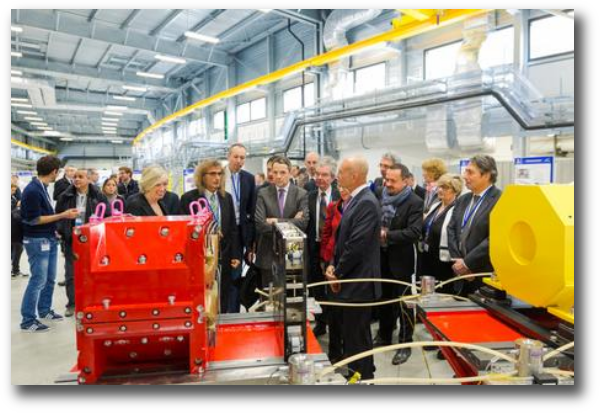
\includegraphics[scale=0.5]{ESRF-people1}};
  \node at (1,3.1) {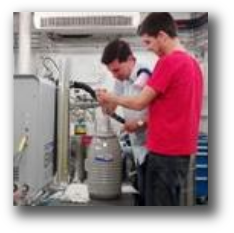
\includegraphics[scale=0.5]{ESRF-people2}};
  %\node at (3.3,1.15) {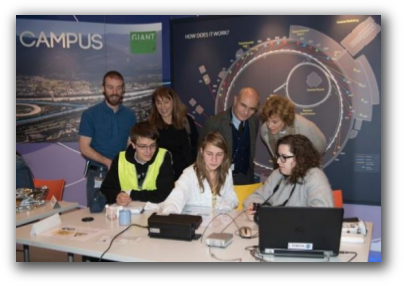
\includegraphics[scale=0.5]{ESRF-people3}};
  \node[NEELblue1,anchor=west,text width=14em] at (-0.2,4.05) {\footnotesize \texttt{\#weekendusers} Express experiments\\%
    \vspace{-0.4em}\hspace{6.7em} for better health.};
  \node[anchor=west,text width=8em] at (1.9,2.88) {\tiny 19-09-2016\\\vspace{4pt}%
    \begin{spacing}{0.2}
    A synchrotron is a particular type of cyclic particle accelerator, descended from the cyclotron...
    \end{spacing}};
\end{tikzpicture}
\end{column}%
\hfill%
\begin{column}{0.5\textwidth}
\begin{block}{\LARGE Audiences and aims}
\setlength{\leftmargini}{0.9em} % Control the left margin!
\begin{itemize}
  \item The scientific community -- to provide information about ESRF activities.
  \item The ESRF/synchrotron community -- to provide information, and strengthen the community of users.
  \item Science and technology decision makers -- to promote ESRF activities and increase the impact of ESRF projects.
  \item The general public, young people -- to foster engagement with scientific issues.
\end{itemize}
\end{block}
\end{column}%
\end{columns}

\end{frame}

%%%%%%

\begin{frame}{NEEL {\LaTeX} Beamer template}

The following packages are needed for this theme:

\begin{itemize}
\item Beamer
\item TikZ
\end{itemize}

If your {\LaTeX} distribution is installed without them, please update and install these packages.

The following colours are defined in the template:
\begin{center}
\begin{tikzpicture}[rounded corners=3pt]
  \foreach \x/\y/\name in {
      0/0/NEELblue1,
      1.5/0/NEELblue2,
      3/0/NEELgreen,
      4.5/0/NEELcyan,
      6/0/NEELmagenta,
      7.5/0/NEELyellow,
      0/-1.5/NEELorange1,
      1.5/-1.5/NEELorange2,
      3/-1.5/NEELorange3,
      4.5/-1.5/NEELdarkerGrey,
      6/-1.5/NEELmidGrey,
      7.5/-1.5/NEELlightGrey,
  } {
    \fill[\name] (\x,\y) rectangle (\x+1.2,\y+1.2);
  };
\end{tikzpicture}
\end{center}

No more than three secondary colours should be used together in a composition. Grey will complement all of the colours.

\end{frame}

%%%%%%

\begin{frame}[t]{Video playback}

\begin{itemize}
  \item Videos can be played from within the presentation:
\end{itemize}
\begin{center}
  \href{run:ID16A.mp4?autostart&loop}{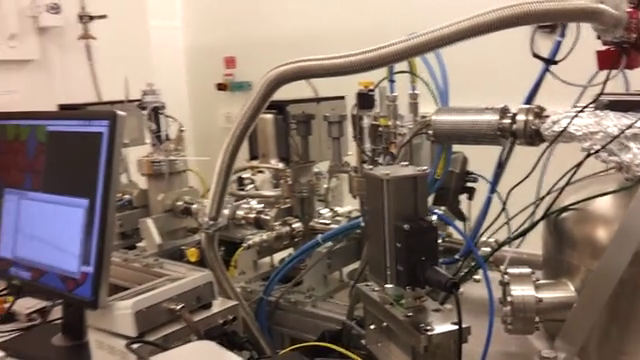
\includegraphics[height=0.23\textheight]{ID16A_snap}}
\end{center}
\begin{itemize}
  \item This may or may not work on Windows machines, but tested to work on Linux.
  \item This requires a supporting presenter, \emph{e.g.} \textbf{pdfpc}.
  \item Also, at least the ``base'', ``good'', ``bad'', and ``libav'' GStreamer plug-ins should be installed.
  \item The video file should be in the defined path (it is not embedded into the presentation, but linked to it).
  \item If for any reason the video will not play, the embedded image will be displayed statically instead.
\end{itemize}

\end{frame}

%%%%%%

\begin{frame}[t]
\frametitle{Tips \& tricks}
\framesubtitle{This is a slide subtitle (optional!)}

\begin{itemize}
  \item For uncovering content in stages check out:
  \begin{itemize}
    \item The \codebox{\texttt{{\textbackslash}pause}} option
    \item \codebox{\texttt{{\textbackslash}includegraphics<1>}}, \codebox{\texttt{{\textbackslash}includegraphics<2>}}, ...
    \item \codebox{\texttt{{\textbackslash}only<1>}}, \codebox{\texttt{{\textbackslash}only<2>}}, ...
    \item \vspace{0.2em}Within TikZ pictures:
    \begin{itemize}
      \item \codebox{\texttt{{\textbackslash}uncover<1>}}, \codebox{\texttt{{\textbackslash}uncover<2->}}, \codebox{\texttt{{\textbackslash}uncover<3>}}, ...
      \item This works for any element in any sequence.
    \end{itemize}
    \item etc...
  \end{itemize}
  \item A great tool for showing {\LaTeX} presentations is \textbf{pdfpc}.
  \begin{itemize}
    \item It supports screen spitting, with overview of all the slides
    \item Support for videos in pdf presentations
    \item Support for notes
    \item A timer
    \item Open source software
    \item Command line interface
  \end{itemize}
  \item A lot of other possibilities to explore -- Beamer is more powerful than it looks!
\end{itemize}

\end{frame}

\end{document}
